\documentclass[12pt]{article}
\usepackage[utf8]{inputenc}
\usepackage[margin = 1in]{geometry}
\usepackage{setspace}
\usepackage{graphicx}
\usepackage{gensymb}
\usepackage{algpseudocode}

\title{Swimming Pool Remote Measurement}
\author{Pranav Chatur\\Department of Computer Science \& Engineering\\The LNM Institute of Information Technology, Jaipur\\Roll No: 20ucs138\\Email: 20ucs138@lnmiit.ac.in}
\date{}

\onehalfspacing
\begin{document}
\maketitle

\begin{center}
    \section*{Abstract}
    The purpose of this paper is to provide a new perspective on monitoring and controlling conditions of a swimming pool. Despite many attempts to tackle this issue, no method uses the concept of multi-agent systems to solve the problem. The paper initially looks into the type of environment and tabulates the parameters associated with the topic. It then looks into previously suggested approaches, their merits and demerits. The paper then starts discussing the solution by taking a hypothetical example of a club wanting to build a remotely controlled swimming pool. It discusses the different agents that are apt for situation and their interactions among themselves and gives a schematic representation of the same. Further, a possible implementation of proposed model is discussed, hardware required is specified and software tools to be used are mentioned and justified. Additionally, few challenges in the implementation and the model itself are stated and possible ways to by-pass them are discussed. The paper ends with emphasizing the points to be noted having Indian context in mind and recommends strategies to make the implementation more relevant and effective in this context.
\end{center}


\section{Introduction}
\textit{Internet of Things (IoT)} is a network of physical items that can connect to the Internet, identify themselves, and communicate with one another to accomplish a shared objective. This technology’s major goal is to share and update data between physical objects in order to achieve optimal performance. \cite{iotDef}

With the advent of IoT and Wireless Sensor Networks (WSN), the facets of using technology have gained a whole new dimension. 
Every particular object available around can be turned into a smart system, one having its own identity and capable of communication. 
Such monitoring and control capabilities alongside a multi-agent agent based paradigm lead to a solid repertoire for creation of an autonomous system capable of adapting to the environment as and when needed. 
Such is the situation of monitoring swimming pools.
\\

%%Define the problem
Swimming is a popular leisure activity for most people in India. Many are daily swimmers and interface with pool waters for a large duration of time. Therefore, it is concerning that, at present, there is a lack of uniformity in the swimming pool sector in India. This is due to the fact that there is no cohesive method in place for collecting and collating data from different pools. Moreover, for places which do have a system in place for data collection, often fail to regulate the conditions of the pool based on the common safety standards, simply because of negligence and lack of sincere staff.\\
These lapses have tremendous implications though. Prolonged exposure to higher levels of chlorine and turbid waters have pernicious effects on the health of an individual. Therefore, it is important to implement a sensor network that is able to perform tests that monitor and control such levels correctly and precisely.

\subsection{Understanding the environment}

A logical approach would be delineating the environment of a swimming pool in an agent-based context. A swimming pool and its surrounding is a fully-observable, cooperative, stochastic, sequential, uncertain, dynamic, continuous, known and multi-agent based environment.\\
Because of such a nature of the environment, there is certain degree of ease when it comes to designing an agent-based solution model as much of the important factors and criteria to measure, monitor and control are already available beforehand. The following sub-section is dedicated to familiarize reader with such factors and parameters.

\subsection{The parameters associated with swimming pool measurement}

The ultimate goal of proposed solution must be to achieve a good water balance. The amount of chemicals in the pool should be exactly the amount that is needed to keep the pool disinfected, good for pool materials and safe for swimming.\\
The primary source of pollution in any pool is from the bathers themselves. Pollutants deposited by bathers into the pool include: sweat, urine, mucus from nose and chest, saliva, hair, cosmetics and scales from skin and faecal matter.
Moreover, when the pool is not in huge for large periods of time, the stagnant water bodies also attracts water-breeding microorganisms alongside pollutants mentioned above.\\
In order to prevent such pathogens from creating ecosystems in the pool, artificial chemicals like \textit{calcium hypochlorite $Ca(ClO)_2$} are added to increase Chlorine levels are disinfect the pool.\\
Turbidity of water also plays a critical role here. The more turbid the water the more particles there are to shield microorganisms from the disinfectant. $Al_2(SO_4)_3$ is used for regulating turbidity.\\
The pH of pools for residential societies in India as mentioned in \cite{myGate}, should be ideally between 7.2 and 8. Higher than that, swimmers are likely to develop skin rashes, and lower than that can sting their eyes. $NaHCO_3$ and $HCl$ are used to moderate this parameter.\\
Furthermore \textit{Total Dissolved Solids (TDS)} levels of above 1000mg/L or hardness value of below 40mg/L (as $CaCO_3$) can corrode the pool material. A hardness level of above 150mg/L can cause scaling to occur.\\
Lastly, the temperature of the water, for the comfort of the swimmer, can be moderated with the effective use of water heaters present with the pool's specifications.\\
Table 1 summarises all of the above mentioned factors.
\begin{table}
\begin{center}
\begin{tabular}{|l|l|l|l|}
    \hline
    \multicolumn{1}{|c}{Sr.no} & \multicolumn{1}{|c}{Parameter} &\multicolumn{1}{|c}{Purpose}&\multicolumn{1}{|c|}{Control Measure}\\
    \hline \hline
    1. & Chlorine Levels & Disinfect pool & \begin{tabular}{l}Increase: Add $Ca(ClO)_2$ \\ Decrease: Add source water\end{tabular} \\
    \hline
    2. & Turbidity & Avoid disinfectant shielding & \begin{tabular}{c}Decrease: Add $Al_2(SO_4)_3$\\\end{tabular} \\
    \hline
    3. & pH Value & Prevent skin-related diseases & \begin{tabular}{l}Increase: Add $NaHCO_3$ \\ Decrease: Add $HCl$\end{tabular} \\
    \hline
    4. & TDS Levels & Prevent material corrosion & \begin{tabular}{c}Decrease: Add source water\\\end{tabular} \\
    \hline
    5. & Hardness & Prevent material damage & \begin{tabular}{l}Increase: Add $CaCl_2$ \\ Decrease: Add source water\end{tabular} \\
    \hline
    6. & Temperature & Provide comfort & \begin{tabular}{l}Increase: Turn Heater On \\ Decrease: Turn Heater Off\end{tabular} \\
    \hline
    \hline
\end{tabular}
\end{center}
    \caption{Important Pool Parameters to Monitor and Control}
    \label{parameter_table}
\end{table}
\\The following section briefly describes previous efforts made to tackle remote monitoring of swimming pools.

\section{Related Work}
The authors of \cite{IDBMS} developed a database management system for swimming pools consisting of extremely precise sensors collectively communicating with nodes. But accurate sensors are extremely expensive hence the solution isn't feasible in Indian sub-context.\\
\\
In South Africa, few researchers \cite{southAfrica}, have perform tests on chlorine levels and pH and make necessary adjustments, all while keeping it cost effective and energy efficient. The scope of the implementation, though, can be largely expanded.\\
\\
Elsewhere, an android mobile application was created for real-time monitoring of swimming pool allowing for faster data analysis, through savvy boats. This solution furthered allowed to clean the pool off of leaves and wastes on the surface of the water. Refer \cite{paper2} for more details.\\
\\
Authors \cite{paper3} made use of National Instruments hardware and its software package LabView for automatic data analysis, remote monitoring and control as well as online connectivity. They also went on to research for development of a biosensor to detect E.coli, best indicator of contamination in water.\\
\\
Finally the one most closely related with the implementation being discussed in this paper is \cite{paper1}. It uses Wireless Sensor Networks (WSN) and Internet of Things (IoT) alongside with hardware, LoRa and ESP32 and a mobile application to control some actions in the swimming pool, in order to stabilize some required parameters for its good quality.\\
\\
Despite all of these efforts, none of them adopt a multi-agent based approach to tackle the issue at hand. This is where the solution proposed in this paper differs from the above implementations. By having multiple agents, capable of social interactions, autonomously functioning according to their performance measures while simultaneously interacting with other agents to achieve the desired goal is a better approach in terms of modular architecture and power efficiency.

\section{Topic Discussion of Proposal}

    \subsection{Periwinkle Club: A Smart Swimming Pool}
    %0.5 pages
    Consider, Periwinkle club, a hypothetical club which wants to create an environment of \textit{smart swimming pool}, i.e. a swimming pool equipped with autonomous capabilities for monitoring and controlling important parameters, while also sending information to the coordinator of the club at any and all times.\\
    The dimensions of the pool will be that Olympic-size swimming pool, i.e. 50 metres long and 25 metres wide with a depth ranging from 2 metres to 3 metres.\cite{poolDimension}\\
    Furthermore, the pool will be installed with additional sensors and actuators as the per the agents designed which will be discussed in the upcoming sub-sections.
    
    \subsection{Agents and their interactions}
    %0.5 page
    Considering the above parameters, proper designing of the agents is absolutely crucial for the solution to be power efficient and cost effective hence implementable.\\
    \\
    Based on Table 1, it is clear that a \textit{Chemical Dispenser} agent is a must. This agent is designed to be a \textit{Procedural Reasoning Agent} \cite{Wooldridge}. This agent's role (\textit{body}) would be to store and release the desired chemicals ($Ca(ClO)_2$, $Al_2(SO_4)_3$, $NaHCO_3$, $HCl$ and $CaCl_2$) when needed. It communicates with other agents to identify when to release which chemicals (\textit{Context}) and when to stop (\textit{Goal}).\\
    Naturally the next agent, would be a sensor-based \textit{Inductive Reasoning Agent} \cite{Wooldridge}, say \textit{Quality checker} agent. It checks the quality of water at variable intervals (which it learns through bottom-up reasoning) and signals Chemical Dispenser and other agents when action is needed.\\
    Another agent is needed to supply the pool with extra water from a nearby source of water as and when needed, say \textit{Water supplier} agent. This agent can also be designed to be an inductive reasoning agent so that the periodicity of water level depletion can be exploited to automate the process.\\
    The forth agent needed would be the one that checks the temperature and water levels of the pool, say \textit{Amount checker} agent. It interfaces with the pool and Water supplier agent (and a heater agent discussed in next paragraph) and signals other agents when water needs to be supplied to the pool or when the water needs to be turned on. Naturally, it is best to designed it as a procedure-based reasoning agent where context and goal are obtained through sensors and goal is communicating with other agents.\\
    The last agent needed to complete our multi-agent based environment is simply a \textit{Water Heater} agent. It communicates(Context) with Amount checker to identify when to turn the heater on (Body) and when to turn it off(Goal).\\
    \\
    Above are the 5 agents necessary for completely automating a swimming pool ecosystem.\\
    Figure \ref{diag} depicts a schematic representation of the agents and their interactions among themselves.
    \begin{figure}
        \centering
        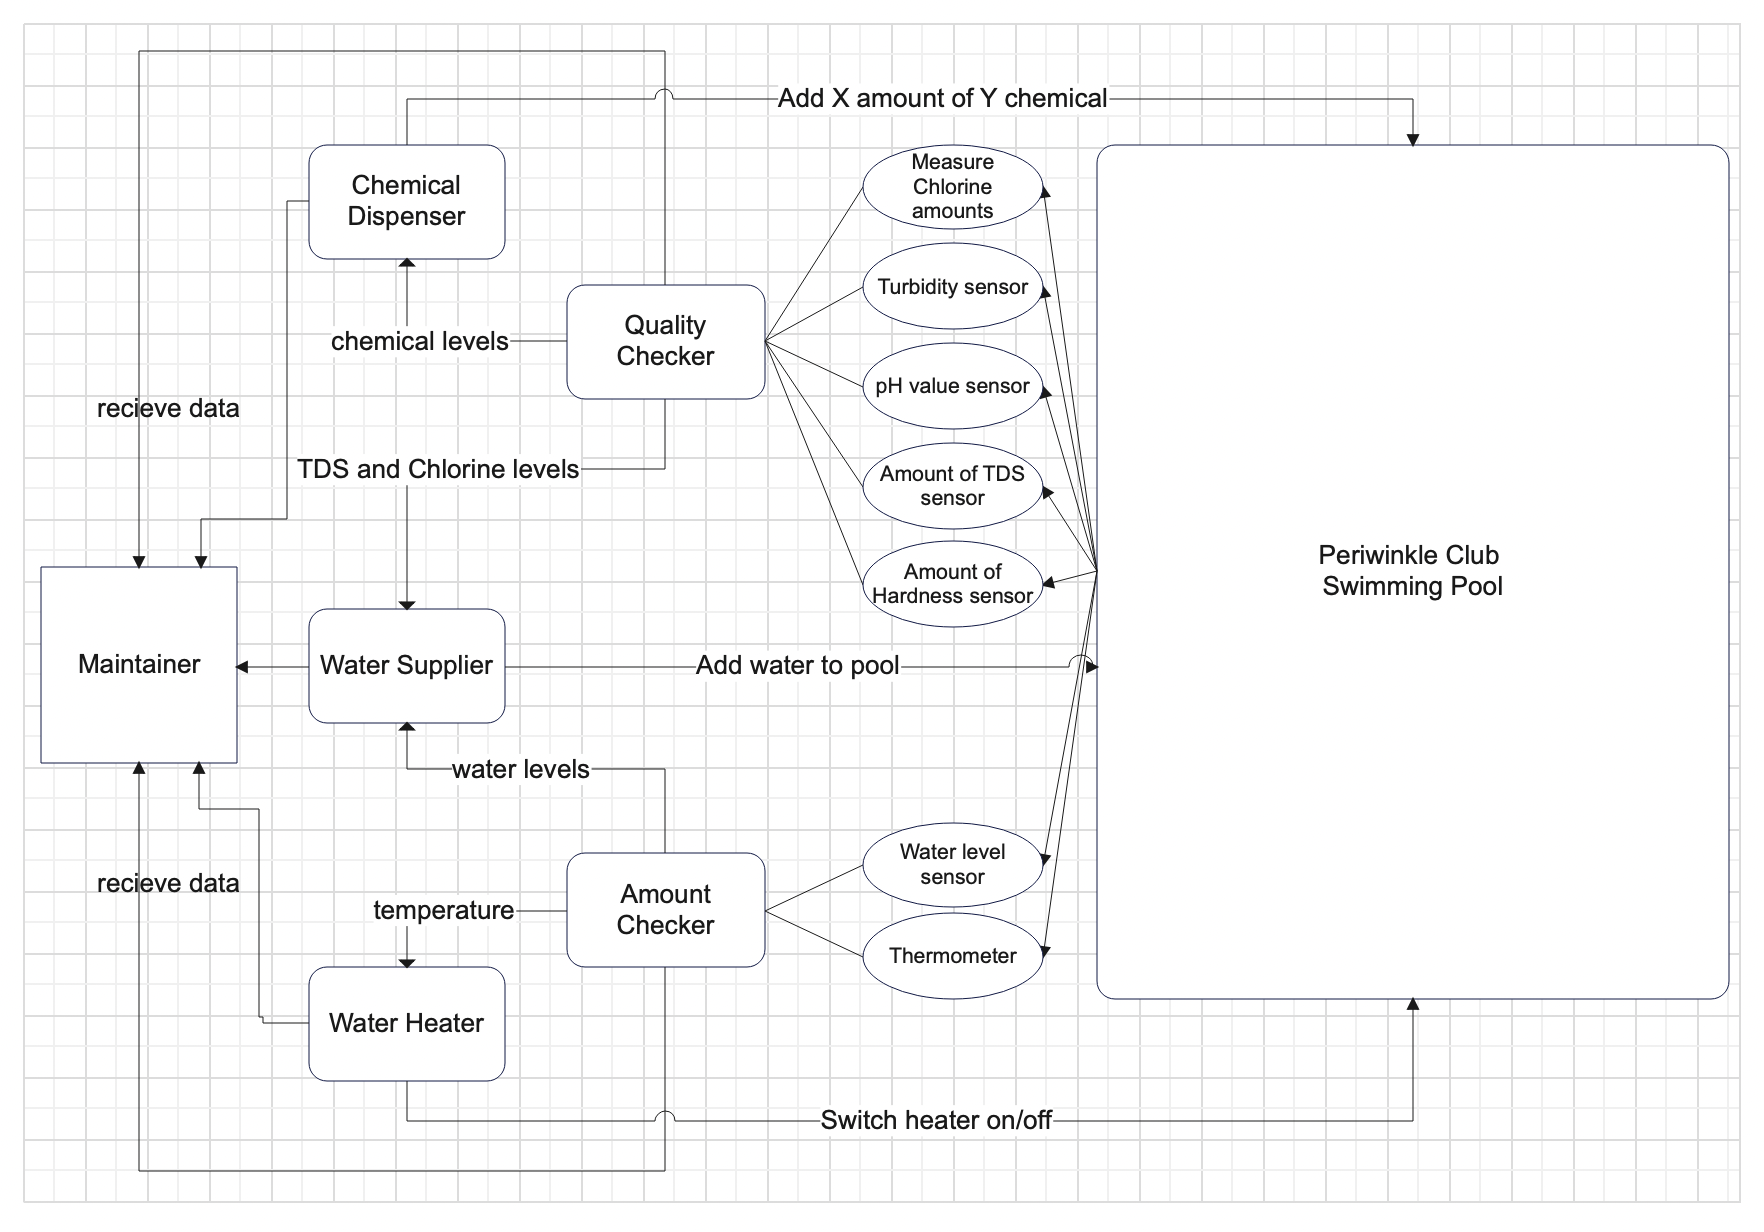
\includegraphics[width = \textwidth]{AgentInteraction}
        \caption{Schematic representation of the proposed solution}
        \label{diag}
    \end{figure}
    \\
    Such a subsystem is placed at multiple locations in the Periwinkle swimming pool, covering the corners as well as the center of the pool to ensure greatest amount of coverage. Next section discusses ways to realise this model.
    \subsection{Implementation: Hardware and Software}
    %1 page
    %
    To implement the model presented in Figure \ref{diag}, this section proposes a hardware-software interface which uses a combination of sensors, databases and necessary interfaces to realise the model as proposed.
    
    \subsubsection{Hardware}
    The hardware required for the implementation primarily includes sensors as evident in the schematic representation.
    Following are the list of sensors that are apt for the this problem.
     \begin{enumerate}
        \item SZ283 is an amperometric chlorine sensor is designed to give continuous or online Chlorine measurements. An Amperometric system measures a change in current directly proportional to the chlorine present in the sample. \cite{chlorine}
        \item SEN0189, a turbidity sensor, that detects water quality by measuring the levels of turbidity. It uses light to detect suspended particles in water by measuring the light transmittance and scattering rate. \cite{turbidity}
        \item SEN01161 is an analog pH meter kit, that allows pH readings from 0 to 14. \cite{pH}
        \item SEN0205, a liquid level sensor that operates using optical principles, can be used to measure water levels. It has good sensitivity and no need for mechanical parts. \cite{level}
        \item DS18B20 is a digital thermometer which can read temperatures as cold as -55\degree C to 125\degree C. \cite{thermo}
         
     \end{enumerate}
    
    \subsubsection{Software}
    Software part of the solution involves collection of data from the available hardware, verifying and cross-checking the data with an existing database of values that are deemed safe and deal with communication among agents.\\
    \\The hardware needed was discussed in the previous section. Any distributed database, like MongoDB or CassandraDB, can be used for the purpose of storing the data and comparing it with advised values of the parameters.\\
    A programming language like Java is particularly helpful for implementation of software interfaces, mainly due to 2 reasons.
    
    \begin{enumerate}
        \item \textit{Java Agent Development Framework(JADE)}.\\ 
        JADE is a software framework for the development of intelligent agents, implemented in Java. It simplifies the implementation of multi-agent systems through a middle-ware through a set of graphical tools that support the debugging and deployment phases.
    
        \item Android support for user\\
        As Java is the preferred language for Android development, there will be sufficient ease in developing an Android application through which user will be notified of any and all updates about the pool by the agents at regular intervals of time. 
    \end{enumerate}
    
    \subsection{Challenges in implementation}
    The proposed solution is rather easy to implement due to the nature of the problem itself being easy. The hard part, though is implementing the solution in a way that is sustainable, foolproof, maintainable and easy to locate errors in the system.\\
    \\
    The approach suggested here fails to deal with a rare yet important scenario. As all the parameters that were listed in Table 1, aren't visible to naked eye, it is impossible to determine whether an agent or subsequently one of its sensors have failed or not.\\
    Completely automating systems having erroneous sensors can lead to ineffable disasters. Thus among others, the major issue of this approach is when an agent or its sensor fails.\\
    \\
    There are a few solutions for this drawback though which can be implemented right from the get go itself.
    As there are multiple such subsystems present in the swimming pool, it could happen that one of the many sensors fail and in such a case, algorithms could be written to detect inconsistencies in the data and ignore requests that obviously seem to have come from a faulty sensor or agent, instead inform the user of a faulty agent.\\
    Furthermore, a safety check mechanism, like requiring user authentication, when about to execute an action that would be considered rather dangerous in normal circumstances.
    
    \subsection{Emphasis on Indian context}
    %0.5 pages
    The problem taken on many new dimensions when Indian context is taken into account.\\
    Primarily, the season patterns in India are different from rest of the world because of the monsoon rains. Rains are particularly disturbing for open-roof swimming pools as they significantly change the properties of water.\\
    To avoid overworking the agents, agents can be rested until rains stop. An even opulent approach could be designing a shutter over the surface of the pool to pull over as soon as heavy rains start to further minimize energy consumption in maintenance of pool.\\
    \\
    Another problem that is particular to India are the crowds. As India is the one of the most populous country, swimming pools are over-populated during evenings. Hence if the sensors aren't guarded properly, then it could lead to increased sensor failures because of taking heavy physical damage from the crowds. Hence sensor protection is especially important in India.\\
    Among others, improper maintenance schedules and failure to replace broken sub-systems are yet another set of traits that are rather prevalent in India. Having periodic maintenance calls in-built into the system so it becomes harder to by-pass the schedules could be one of the possible ways to try and reduce such problems.
    
\section{Conclusion}
The purpose of this paper was to provide a possible approach for monitoring and controlling swimming pools using multi-agent systems, while keeping it simple, efficient and cost-effective. Such a system, if implemented scrupulously, has the capacity to enhance quality of lives for many individuals as well as reduce labour workload and consumption of natural resources to achieve a higher level of efficiency. Although the system is designed for swimming pools, the same model can easily be extended to other public amenities keeping the same spirit intact. 

\begin{thebibliography}{}

\bibitem{iotDef}
H.N. Saha, A. Mandal and A. Sinha,
``Recent trends in the Internet of Things",
\textit{IEEE 7th annual computing and communication workshop and conference (CCWC)}, 2017

\bibitem{myGate}
Team MyGate. (March 21, 2022)
\textit{Swimming Pool Rules and Regulations in a Residential Society}
[Online]. Available: https://mygate.com/blog/swimming-pool-rules-gated-community

\bibitem{IDBMS}
J. M. Marais, D. V. Bhatt, G. P. Hancke, and T. D. Ramotsoela,
``A web-based swimming pool information and management system,"
\textit{IEEE Int. Conf. Ind. Informatics}, pp.980-985, 2017.

\bibitem{southAfrica}
R. Gouws and A. Nieuwoudt,
``Design and cost analysis of an automation system for swimming pools in South Africa,"
\textit{(DUE), 2012 Proc. 20th, no. 2}, pp. 9–15, 2012.

\bibitem{paper2}
S.A. Asiri,
``Smart solutions for monitoring, control, and safety of swimming pools using a savvy boat",
\textit{Measurement and Control}, 55(7-8):603-615, 2022.

\bibitem{paper3}
P. Duffy, G. Woods, S. O'Hogain, J. Walsh, C. Caplier,
``On-Line Realtime Water Quality Monitoring and Control for Swimming Pools", \textit{International Manufacturing Conference}, 
Trinity College Dublin, Ireland, September, 2009.

\bibitem{paper1}
G. Simoes, C. Dionisio, A. Gloria, P. Sebastião, N. Souto. 
``Smart System for Monitoring and Control of Swimming Pools". 
\textit{WF-IoT.2019}. 829-832. 10.1109, 2019. 

\bibitem{poolDimension}
M. Zrinjski, D. Barković, K. Matika.
``Precise Measurement and Analysis of the Olympic-size Swimming Pool Lanes Distance". 
\textit{Geodetski List}. 75 (98). 45-58. 2021.

\bibitem{Wooldridge}
M. Wooldridge.  
\textit{An Introduction to MultiAgent Systems}, 2nd. ed. Wiley Publishing. 2009.

\bibitem{chlorine}
Automated Water \& Effluents Ltd,
\textit{Chlorine Instruments for Water Treatment Applications}[Online].
Available: https://www.awe-ltd.co.uk/products/chlorine.html

\bibitem{turbidity}
DFRobot, (2008).
\textit{Turbidity sensor SKU: SEN0189.}[Online]. Available: https://www.dfrobot.com/wiki/index.php/Turbidity\_sensor\_SKU:\_SEN0189. 
[Accessed: 10-Dec-2018].

\bibitem{pH}
DFRobot, (2008).
\textit{PH meter(SKU: SEN0161)} [Online]. Available: https://www.dfrobot.com/wiki/index.php/PH\_meter(SKU:\_SEN0161). [Accessed: 10-Dec-2018].

\bibitem{level}
DFRobot, (2008).
\textit{Liquid Level Sensor-FS-IR02 SKU: SEN0205}[Online].
Available: https://www.dfrobot.com/wiki/index.php/Liquid\_Level\_Sensor- FS-IR02\_SKU:\_SEN0205. [Accessed: 10-Dec-2018].

\bibitem{thermo}
M. Integrated, (2018).
\textit{DS18B20 Datasheet} [Online]. 
Available: https://datasheets.maximintegrated.com/en/ds/DS18B20.pdf.[Accessed: 07-Dec-2018].

\end{thebibliography}


\end{document}